\documentclass{article}
\usepackage{tikz}
\pagestyle{empty}
%---------------------------------
\begin{document}

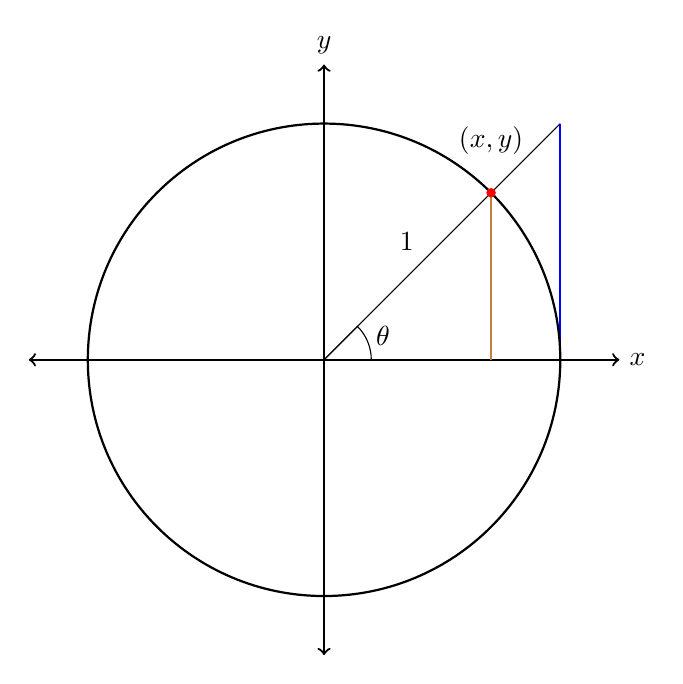
\begin{tikzpicture}[scale=3]
\draw (0,0) -- (2mm,0mm) arc (0:45:2mm) -- cycle; %angle arc for the triangle
\draw[<->, thick] (-1.25,0) -- (1.25,0) node[right]{$x$}; %x-axis and it's label
\draw[<->, thick] (0,-1.25) -- (0,1.25) node[above]{$y$}; %y-axis and it's label
\draw (0,0) -- (1,1); %line from origin to (1,1)
\draw[thick, brown] (.7071,0) -- (.7071,.7071); %brown line 
\draw[thick, blue] (1,0)--(1,1);   % blue line
\draw[black, thick] (0,0) circle (1cm); %The circle
\filldraw[red] (.7071,.7071) circle (.5pt); %the red dot at point (x,y)
\draw (.25,.1) node {$\theta$}; %label the angle theta
\draw (.35,.5) node {$1$}; % label of the radius
\draw (.7071,.83) node[above] {$(x,y)$}; %label (x,y)
\end{tikzpicture}

\end{document}


